\section{Experiments and Results}
\label{sec:experiments}

\subsection{Setup}
\label{sec:setup}

All learned models are trained on the 331 training images, selected on the 66 validation images,
and evaluated once on the 73 test images (Section~\ref{sec:data}). Hyperparameters are identical
for all MIL variants (Section~\ref{sec:mil}); every MIL result is the mean $\pm$ standard deviation
over seeds 42, 43 and 44. As references, predicting the training mean (7.38\,\%) or median
(5.0\,\%) for every image gives a validation MAE of 5.45 / 5.41 and a test MAE of 4.45 / 4.01.
A model has to beat these numbers to be useful.

\subsection{Classical computer vision}
\label{sec:res-classical}

Each classical component was checked by manual review of stratified training/validation samples
(never test images) with overlays of every detection. Table~\ref{tab:classical} summarizes the
outcome, and Figure~\ref{fig:qualitative} shows examples.

\begin{table}[tb]
\centering
\small
\caption{Manual audits of the classical components (training/validation images only).}
\label{tab:classical}
\begin{tabular}{@{}llll@{}}
\toprule
Component & Sample & Result & Decision \\
\midrule
Frame detection + crop            & 30 images  & 30/30 approved             & used \\
Plant-region proposal             & 30 images  & 30/30 approved (191 regions)  & used \\
Plant-mask area weights $A_i$     & 40 images  & 40/40 usable               & used \\
Direct damage: leaf mask, pitting & 40 images  & 40/40 acceptable           & exploratory \\
Direct damage: shot holes         & 40 images  & 0/40 usable                & rejected \\
Soil-aware hole rule (CIELAB)     & 20 images  & inconsistent across soils  & rejected \\
Leaf/cotyledon counting           & 8 patches  & systematic over-counting   & rejected \\
RF-DETR hole/pitting detector     & 8 val.\ images & mAP@50 3.5\,\%         & exploratory \\
\bottomrule
\end{tabular}
\end{table}

\paragraph{Frame and plant regions work.} The frame was found in all audited images, and the plant
masks were judged a good approximation of visible leaf area in all 40 images, so they are safe to
use as MIL weights. The green mask does, however, miss strongly discoloured tissue.

\paragraph{Direct damage measurement fails on holes.} Against the expert score, the direct damage
percentage reaches Spearman $\rho = 0.64$ (Pearson $r = 0.46$, $n=40$), but this comes almost
entirely from pitting: the pitting share alone gives $\rho = 0.63$, the hole share only $0.20$.
In manual review the hole detections were unusable in all 40 images, because dark soil seen
through a hole, dark soil next to the leaf and brown pitting have nearly the same colour. The
soil-aware rule did not resolve this. The measurement also underestimates damage by more than an
order of magnitude (mean 0.55\,\% vs.\ 10.2\,\% expert score), mostly because eaten leaf edges
cannot be measured from the remaining leaf shape (Figure~\ref{fig:qualitative}b).

\paragraph{Leaf counting fails because of the damage.} A convexity-defect lobe counter split a
single damaged cotyledon pair into three or four ``leaves'': a feeding notch at the leaf edge is
geometrically indistinguishable from the notch between two leaves. The damage we want to measure
thus breaks the feature, most of all at BBCH10.

\paragraph{RF-DETR: a pipeline bug, then a weak signal.} The first detector reached only
0.4\,\% mAP@50, which we initially attributed to too little data. Plotting the tiled ground truth
revealed the real cause: the tiling script loaded images with automatic EXIF rotation (36 of the 40
images are rotated by 180$^\circ$), while the box coordinates referred to the unrotated image, so
almost every box pointed at soil. After the fix, mAP@50 rose to 3.5\,\% (peak 10\,\% during
training), and predictions now lie on real leaf damage (Figure~\ref{fig:qualitative}c). With only
283 training boxes on $\sim$18\,px objects, and only 61 for pitting, the detector remains far from
usable; we estimate that 150--300 annotated images per class would be needed. The general lesson is
to check a negative result for pipeline bugs before blaming the amount of data.

\begin{figure}[tb]
\centering
\setlength{\fboxsep}{0pt}%
\begin{minipage}[b]{0.235\textwidth}\centering
  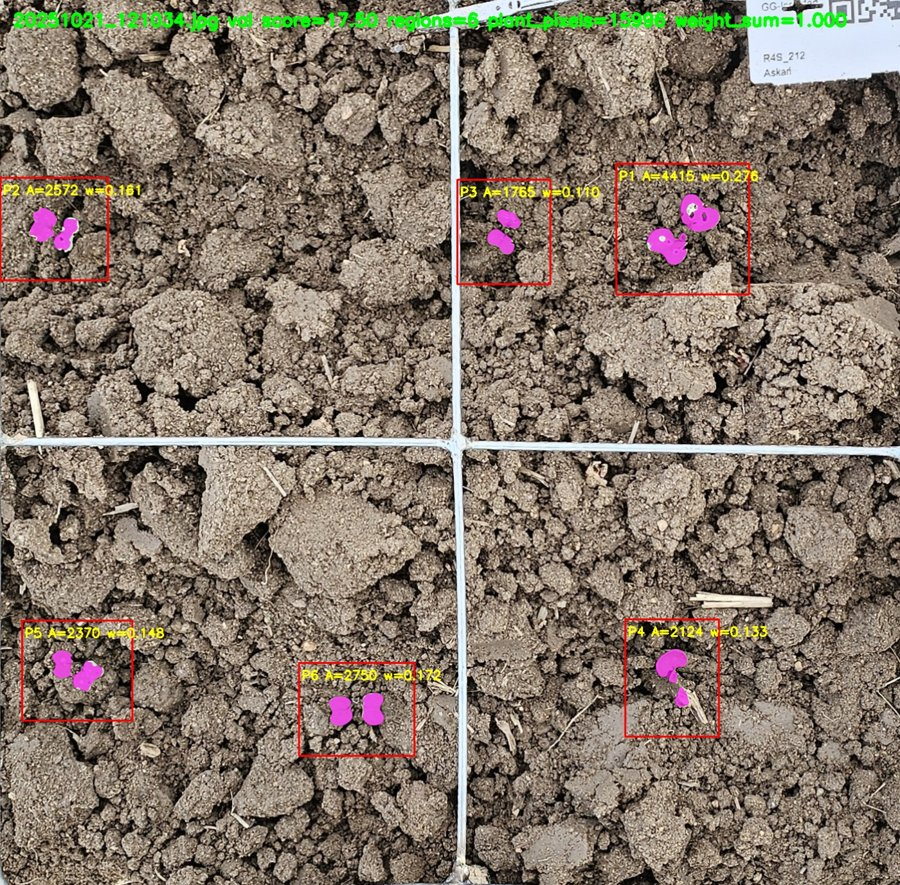
\includegraphics[width=\linewidth]{figures/plant_weights_example.jpg}\\[-1pt]{\small (a)}
\end{minipage}\hfill
\begin{minipage}[b]{0.235\textwidth}\centering
  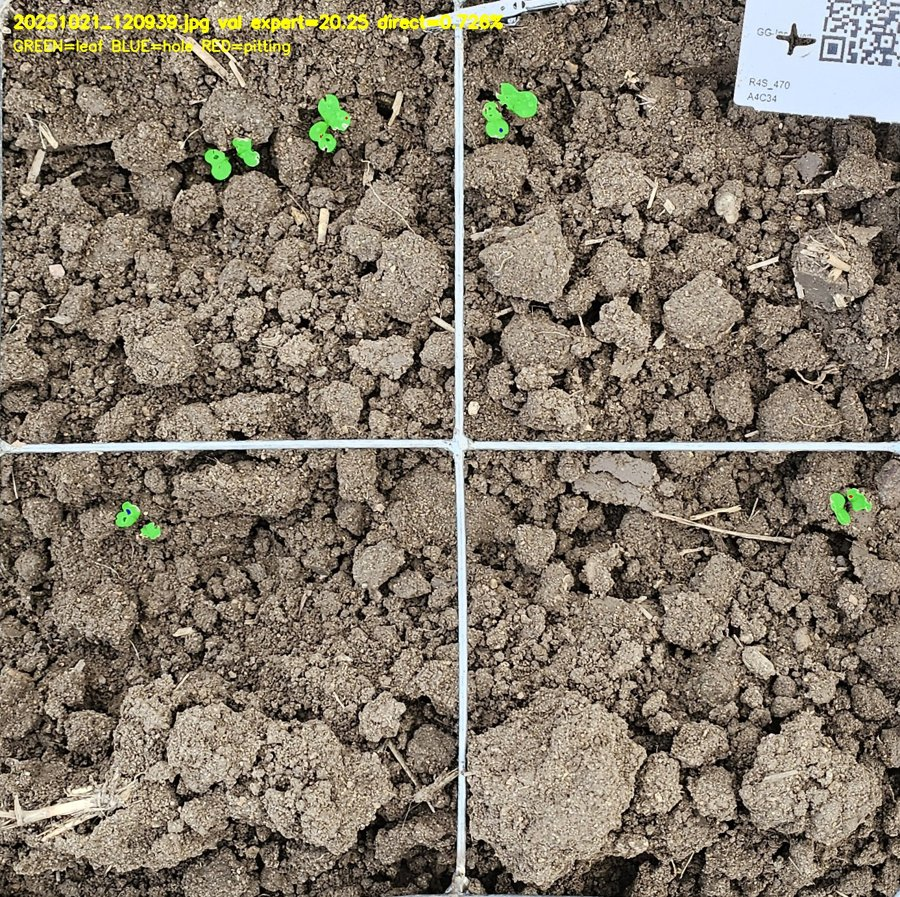
\includegraphics[width=\linewidth]{figures/direct_damage_example.jpg}\\[-1pt]{\small (b)}
\end{minipage}\hfill
\begin{minipage}[b]{0.49\textwidth}\centering
  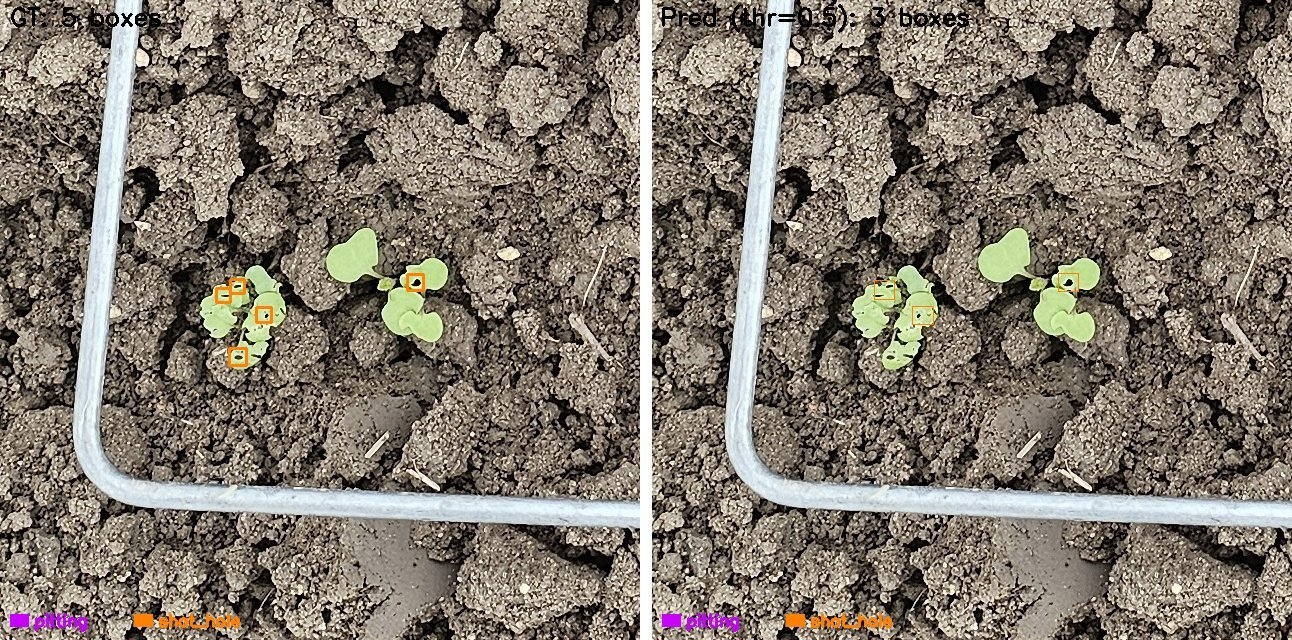
\includegraphics[width=\linewidth]{figures/rfdetr_example.jpg}\\[-1pt]{\small (c)}
\end{minipage}
\caption{(a) Plant regions inside the frame with visible area $A_i$ and weight $w_i$ (expert score
17.5\,\%). (b) Direct damage measurement on an image the experts rated 20.25\,\%: leaf mask in green,
almost no hole or pitting pixels found (0.73\,\%). (c) RF-DETR on a validation tile after the
EXIF fix; left: 5 annotated marks, right: 3 predictions on real damage.}
\label{fig:qualitative}
\end{figure}

\subsection{In-domain scoring: baseline versus MIL}
\label{sec:res-main}

Table~\ref{tab:main} compares all learned models on the Gro\ss-Gerau validation and test sets.

\begin{table}[tb]
\centering
\small
\caption{In-domain results (Gro\ss-Gerau, BBCH10). MIL rows: mean $\pm$ SD over 3 seeds. Pairwise:
share of test pairs with a true difference $\geq 5$ points that are ordered correctly.}
\label{tab:main}
\setlength{\tabcolsep}{4pt}
\begin{tabular}{@{}lccccc@{}}
\toprule
 & \multicolumn{2}{c}{Validation ($n=66$)} & \multicolumn{3}{c}{Test ($n=73$)} \\
\cmidrule(lr){2-3}\cmidrule(l){4-6}
Method & MAE & Spearman $\rho$ & MAE & Spearman $\rho$ & Pairwise \\
\midrule
Constant (training median)        & 5.41 & --    & 4.01 & --     & -- \\
Whole image, DINOv3 (1 seed)      & 5.13 & 0.27  & 4.65 & $-0.11$ & 0.46 \\
\midrule
MIL, uniform pooling              & $2.73 \pm 0.04$ & $0.838 \pm 0.006$ & $\mathbf{2.40} \pm 0.01$ & $\mathbf{0.808} \pm 0.004$ & $0.932$ \\
MIL, ABMIL                        & $2.74 \pm 0.03$ & $0.809 \pm 0.011$ & $2.54 \pm 0.04$ & $0.770 \pm 0.005$ & $0.926$ \\
MIL, gated ABMIL                  & $2.78 \pm 0.02$ & $0.805 \pm 0.011$ & $2.55 \pm 0.03$ & $0.765 \pm 0.007$ & $0.924$ \\
MIL, area-weighted                & $2.69 \pm 0.02$ & $0.853 \pm 0.002$ & $2.62 \pm 0.07$ & $0.763 \pm 0.008$ & $0.924$ \\
MIL, area-weighted + ranking loss & $\mathbf{2.66} \pm 0.04$ & $\mathbf{0.859} \pm 0.001$ & $2.51 \pm 0.05$ & $0.781 \pm 0.002$ & $\mathbf{0.933}$ \\
\bottomrule
\end{tabular}
\end{table}

\paragraph{The whole-image baseline does not learn the task.} Its test MAE of 4.65 is worse than
always predicting the median (4.01), its test correlation is slightly negative, and it orders
only 46\,\% of clearly different image pairs correctly, which is chance level. Its predictions
stay in a narrow band around the mean (SD 2.3 vs.\ 5.6 for the test labels). At $224\times224$ a whole
frame of seedlings shrinks to a few pixels per plant (Figure~\ref{fig:qualitative}b), so the
damage is simply not visible to the backbone.

\paragraph{Plant-level MIL solves it.} All MIL variants reduce the error of the constant predictor
by 35--50\,\% and reach test $\rho$ between 0.76 and 0.81, with over 92\,\% of clearly different pairs
ordered correctly. Since the backbone and the head are the same, the gain comes entirely from
looking at the plants at full resolution instead of the downsampled photograph.

\paragraph{Pooling: small differences, and validation and test disagree.} On validation,
area-weighted pooling was best on both metrics and very stable across seeds, so we selected it
before opening the test set, as the supervisor suggested. On the test set, however, uniform pooling
is clearly better (MAE 2.40 vs.\ 2.62, $\rho$ 0.81 vs.\ 0.76), consistently over all seeds, and the
attention variants lie in between. We report this honestly rather than re-selecting on test. One
plausible explanation comes from how the labels were produced: according to the project partners,
the raters most likely score each plant and \emph{average over plants}, which is exactly uniform
pooling. Area weighting encodes a different target, namely the damaged share of the total leaf
area. With 66 validation and 73 test images, the ranking between the pooling rules is not settled;
what is settled is that fixed pooling is at least as good as learned attention here.

\paragraph{Val--test gap.} For the selected area-weighted model, test $\rho = 0.765$ is lower than
validation $\rho = 0.855$, while the MAE is similar (2.60 vs.\ 2.67). The bootstrap 95\,\% interval
of the test $\rho$ is $[0.62, 0.86]$ and contains the validation value, so with 73 images the gap
is consistent with sampling noise. A second model trained independently by another team member
with the same configuration gives almost identical test results (MAE 2.59, $\rho$ 0.764), which
confirms that the pipeline is reproducible.

\subsection{Ranking-based training}
\label{sec:res-ranking}

Adding the pairwise margin ranking loss to the area-weighted model improves every metric on both
validation and test, and does so for each of the three seeds (last row of Table~\ref{tab:main}):
test MAE drops from 2.62 to 2.51 and test $\rho$ rises from 0.763 to 0.781, with a smaller spread
across seeds. The improvement is small compared with the confidence intervals of a single run, so
we see it as a consistent but modest gain. It supports the idea behind this direction: with
subjective labels, knowing which of two images is more damaged carries useful information beyond
the exact scores. The ranking loss can be combined with any pooling rule; we only tested it with
area weighting.

\subsection{Generalization beyond the calibration set}
\label{sec:res-ood}

\begin{table}[tb]
\centering
\small
\caption{Zero-shot generalization of the area-weighted MIL model (mean over 3 seeds; SD of
$\rho$ $\leq 0.011$). ``Frame'': share of images where the frame was detected. ``Plants'': mean
number of plant regions per image.}
\label{tab:ood}
\begin{tabular}{@{}lrcccccc@{}}
\toprule
 & & & & \multicolumn{2}{c}{Area-weighted} & \multicolumn{2}{c}{+ ranking loss} \\
\cmidrule(lr){5-6}\cmidrule(l){7-8}
Dataset & $n$ & Frame & Plants & MAE & $\rho$ & MAE & $\rho$ \\
\midrule
Gro\ss-Gerau test (reference)            & 73  & 100\,\% & 6.0  & 2.62 & 0.763 & 2.51 & 0.781 \\
Gro\ss-Gerau, raters disagree            & 218 & 99\,\%  & 7.3  & 9.24 & 0.596 & 8.76 & 0.606 \\
Weilburger Grenze (BBCH10)               & 906 & 59\,\%  & 14.3 & 4.32 & 0.031 & 4.29 & 0.070 \\
DSV Asendorf, Trial 1 (BBCH11)           & 897 & 0.1\,\% & 24.4 & 7.73 & 0.264 & 8.24 & 0.239 \\
\bottomrule
\end{tabular}
\end{table}

As the supervisor pointed out, the small test set says little about generalization to other
images. We therefore applied the models without any adaptation to three further sets
(Table~\ref{tab:ood}, Figure~\ref{fig:scatter}).

\paragraph{Images the raters disagree on.} The 218 Gro\ss-Gerau images from plots outside the
training and validation splits whose JLU and GAU scores differ by more than 5 points have the same
field, date and camera as the training data, but noisier and much higher labels (mean 20\,\% vs.\
7\,\%). The model ranks them reasonably ($\rho = 0.60$) but underestimates high damage, since it
has hardly seen scores above 20\,\% during training. Remarkably, the model agrees with each
individual rater ($\rho = 0.50$ with JLU, $0.55$ with GAU) far better than the two raters agree
with each other ($\rho = 0.27$, $r = 0.17$) on these images, where JLU scored on average more than twice as high as GAU (27.4\,\% vs.\ 12.8\,\%). Within its own domain, the model is
therefore at least as consistent as a human rater.

\paragraph{New field trials.} On Weilburger Grenze and DSV the model fails. On Weilburger Grenze it
is essentially uncorrelated with the scores and slightly worse than a constant predictor (MAE 4.32
vs.\ 4.10), and its predictions stay flat across the whole score range. On DSV the rank correlation
is weak ($\rho = 0.26$) and the model overestimates damage (mean prediction 11.8\,\% vs.\ 7.1\,\%),
giving a much higher MAE than a constant (7.73 vs.\ 5.22). No pooling variant does substantially
better on these sets (all $\rho \leq 0.07$ on Weilburger Grenze and $\leq 0.27$ on DSV). Averaging
the three images of each plot, as a breeder would, does not help either (plot-level
$\rho = -0.01$ and $0.23$).

\paragraph{Why the transfer fails.} Inspecting the images shows that the main problem is the
\emph{recording setup}, not only the model (Figure~\ref{fig:ood-examples}). At DSV a different
camera was used, the frame fills the whole photo and has rounded corners, and the frame detector
found it in only 1 of 897 images. At Weilburger Grenze the photos were taken from much farther
away, so the frame covers only part of the image and many plants lie outside it; the frame was
found in 59\,\% of the images. When the frame is missed, the pipeline scores every plant in the
photo (14--24 regions instead of about 6), including plants that the raters did not score, and
each plant is smaller in pixels than in training. Brightness mattered only at DSV, where the darkest third of the images has a clearly higher error (MAE 10.2 vs.\ 6.5 for the brightest third). Even on the Weilburger Grenze images with a detected frame, the correlation stays low
($\rho = 0.17$), so the learned representation itself also transfers poorly. Which part is due to
soil and plant appearance and which to different rating habits at each site cannot be separated
with the available labels.

\begin{figure}[tb]
\centering
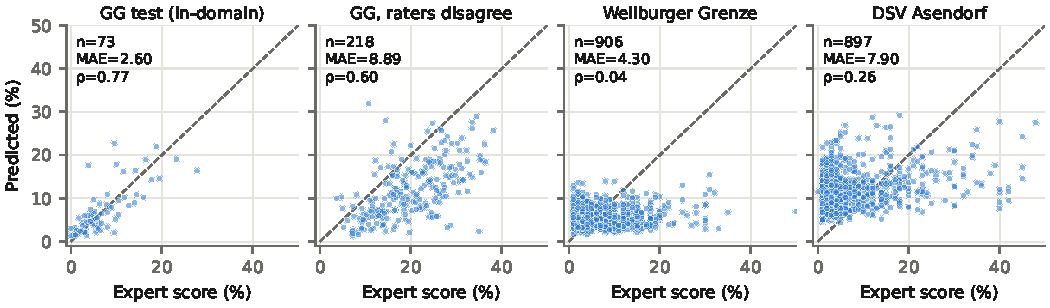
\includegraphics[width=\textwidth]{figures/pred_vs_true.pdf}
\caption{Predicted vs.\ expert score of the area-weighted MIL model (seed 42) on the in-domain test
set and the three generalization sets. Dashed: perfect agreement.}
\label{fig:scatter}
\end{figure}

\begin{figure}[tb]
\centering
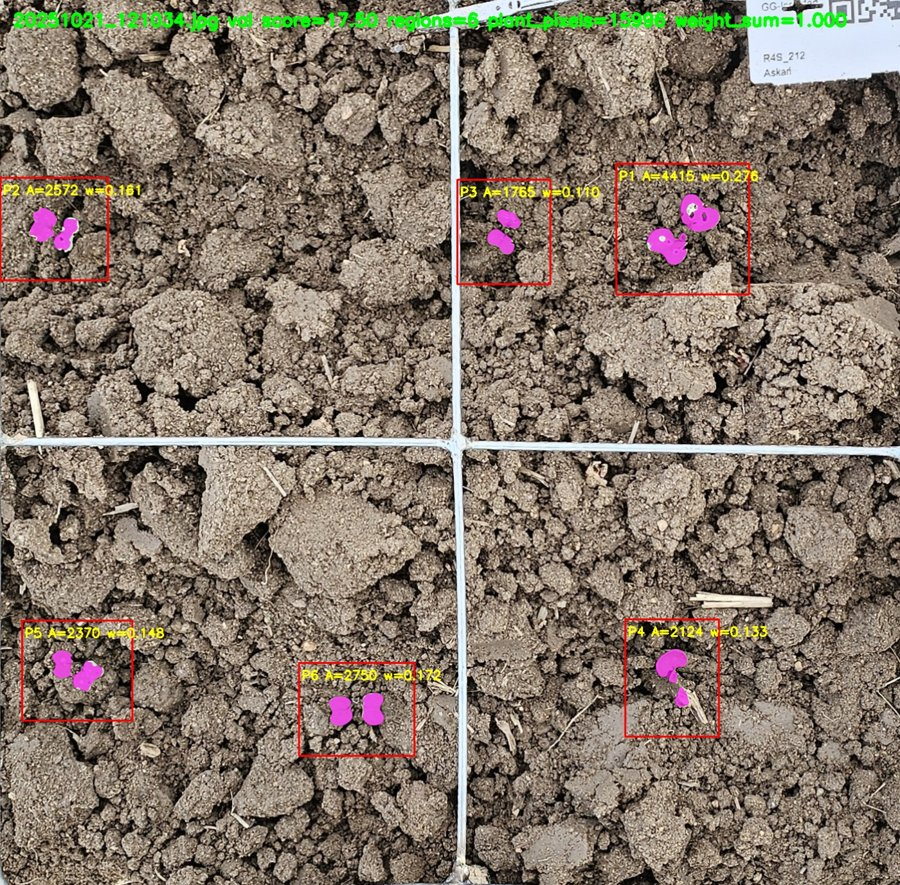
\includegraphics[height=4.2cm]{figures/plant_weights_example.jpg}\hfill
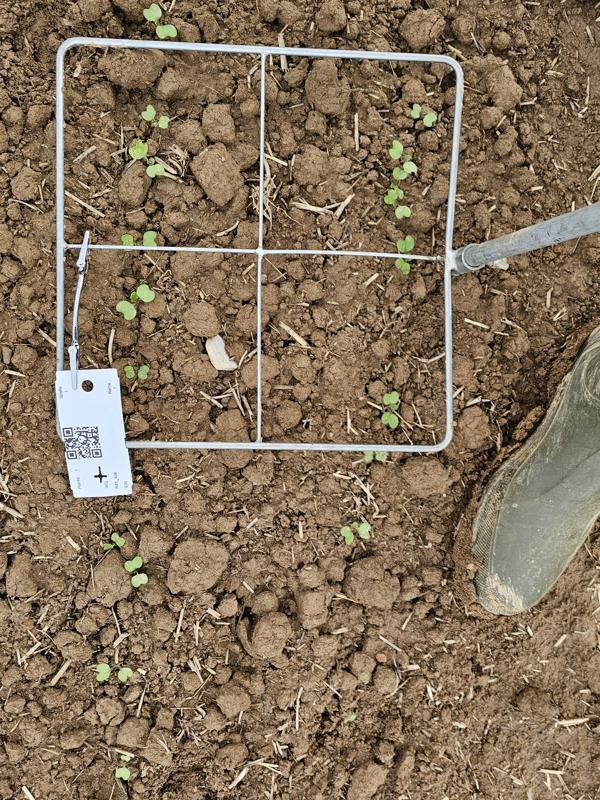
\includegraphics[height=4.2cm]{figures/ood_wg1.jpg}\hfill
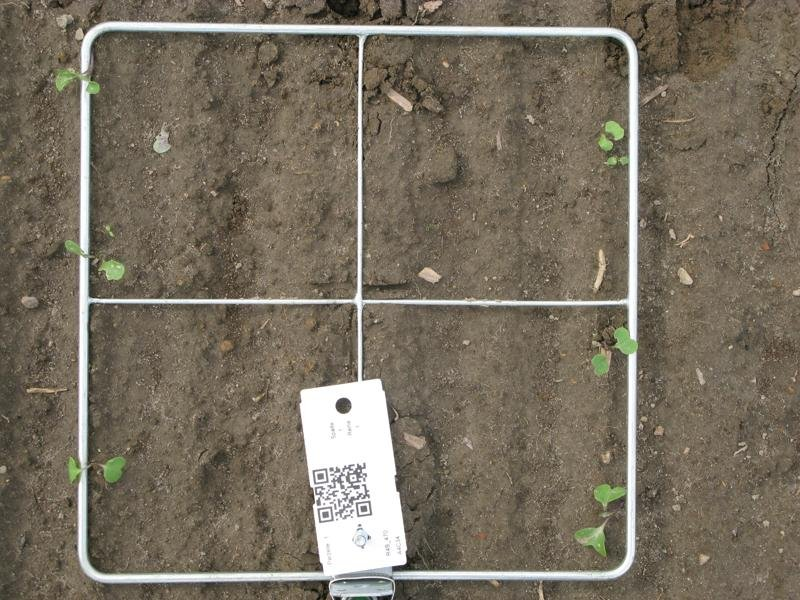
\includegraphics[height=4.2cm]{figures/ood_dsv.jpg}
\caption{Recording setups. Left: Gro\ss-Gerau (training), frame fills the photo, about 6 plants.
Middle: Weilburger Grenze, photo taken from farther away with plants outside the frame. Right: DSV,
different camera and framing; the frame was not detected in 896 of 897 images.}
\label{fig:ood-examples}
\end{figure}
